\section{Durchführung}
\label{sec:Durchführung}

\subsection{Messung bis 1 bar}

Im ersten Aufbau soll die Dampfdruckkurve von Wasser im Druckbereich zwischen $30 \,\unit{\milli\bar}$
und $1000 \,\unit{\milli\bar}$ bestimmt werden.

Der dazu verwendete Versuchsaufbau ist dabei in \autoref{fig:Aufbau1} dargestellt.

\begin{figure}[H]
    \centering
    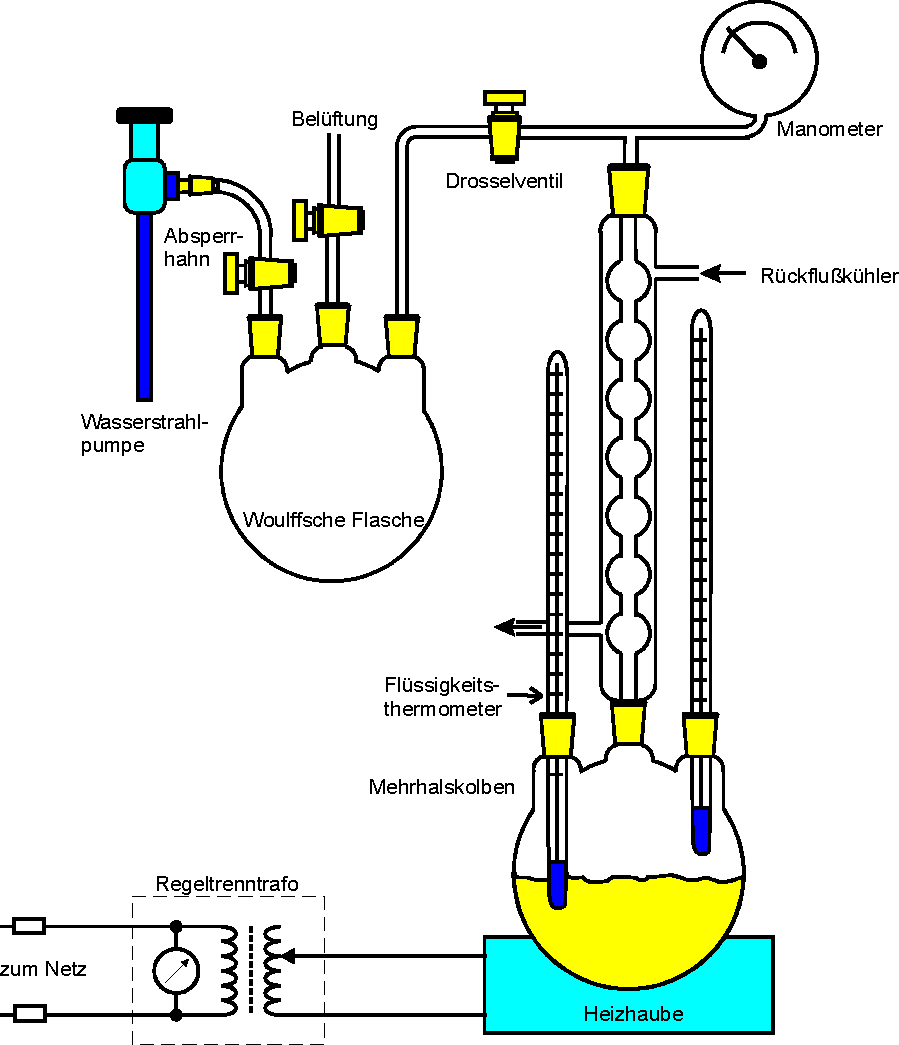
\includegraphics[scale=0.65]{Aufbau1.pdf}
    \caption{Versuchsaufbau für den Druckbereich $p \leq 1 \,\unit{\Bar}$\cite{ap06}.}
    \label{fig:Aufbau1}
\end{figure}

Die Apparatur wird mithilfe einer Wasserstrahlpumpe evakuiert.
Dazu werden der Absperrhahn und das Drosselventil geöffnet sowie das Belüftungsventil geschlossen.
Der Rückflusskühler wird ständig von einer geringen Menge Kühlwasser durchflossen, die Woulffsche Flasche
verhindert bei Abdrehen der Leitungswasserzufuhr ein Eindringen von Wasser in die evakuierte Apparatur. \\

Die Apparatur wird zunächst auf den niedrigsten erreichbaren Druck evakuiert.
Bei tropfendem Kühlwasserzufluss werde pro Temperaturerhöhung von $1 \,\unit{\celsius}$
werde der Druck $p$ abgelesen, bis $1 \,\unit{\bar}$ erreicht sind.


\subsection{Messung bis 15 bar}

Des Weiteren soll auch für den Druckbereich zwischen $1 \,\unit{\bar}$ und $15 \,\unit{\bar}$ die 
Dampfdruckkurve bestimmt werden.
Dazu wird der in \autoref{fig:Aufbau2} dargestellte Aufbau verwendet.

\begin{figure}[H]
    \centering
    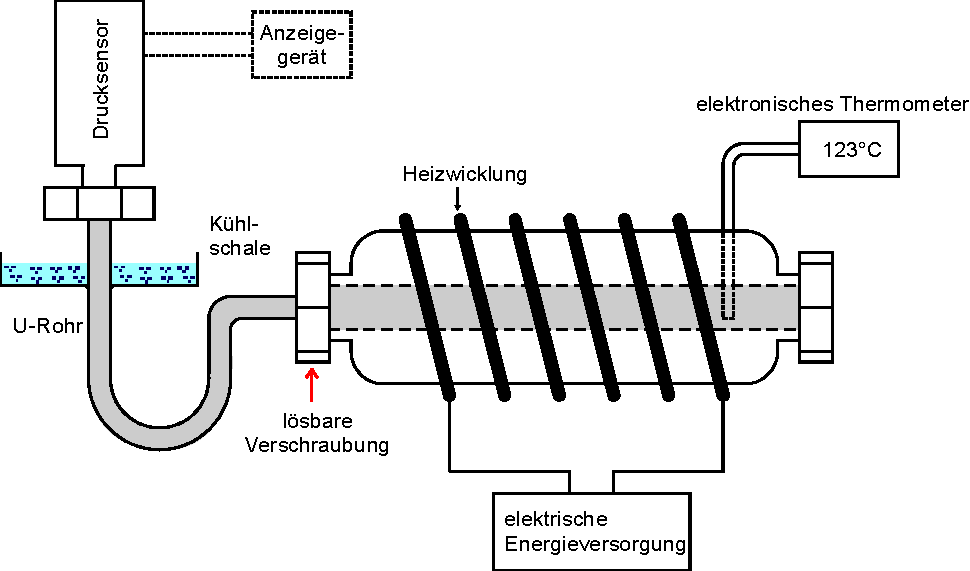
\includegraphics{Aufbau 2.pdf}
    \caption{Aufbau für den Druckbereich $p \geq 1 \,\unit{\bar}$\cite{ap06}.}
    \label{fig:Aufbau2}
\end{figure}

Zur Messung wird lediglich der Heizpilz der Apparatur eingeschaltet, pro $1 \unit{\bar}$ wird jeweils die
Temperatur aufgenommen, bis $15 \,\unit{\bar}$ erreicht sind.


